\title{Energy budget for insects}

\documentclass[12pt]{article}
\usepackage{amsmath}
\usepackage{mathabx}
\usepackage{graphics}
\usepackage[top=1in, bottom=1in, left=1in, right=1in]{geometry}
\usepackage{tabu}
\usepackage[english]{babel}
\usepackage{natbib}
\bibliographystyle{evolution}
\usepackage{rotating}
\usepackage[capitalize, sort&compress]{cleveref}
\usepackage{float}
%\newcommand{\crefrangeconjunction}{--}
%\crefname{section}{Sect.}{Sects.}
%\crefname{equation}{Eq.}{Eqs.}
%\crefformat{equation}{Eq.~#2#1#3}
%\crefrangeformat{equation}{Eqs.~#3#1#4--#5#2#6}
%\crefmultiformat{equation}{Eqs.~#2#1#3}{--#2#1#3}{, #2#1#3}{ and~#2#1#3}
 
% for comments visible in the compiled pdf
%\usepackage{color}
%\definecolor{orange}{rgb}{0.8,0.4,0}
%\newcommand{\eeg}[1]{{\em \color{orange} #1}}

% Tell latex how it can introduce linebreaks if necessary.
\hyphenation{Bar-thol-o-mew}

\begin{document}
\maketitle

\section*{Introduction}
A principal goal in ecology is to describe and understand processes that influence species distribution.
The act of describing and explaining is not often mutually inclusive.
In some cases, things fit naturally.
Abiotic factors can easily correlate with species range.
Temperature isocline matches range limits which provides evidences of range limitiation \citep{Root1988}.
Biotic factors also plays a role in the shaping species range \citep{Krebs2000}.
Various types of interaction within and among trophic level can both expand or contract species distribution.
In the most general case, it is not evident which factor is most important.
Sometimes, several factors are correlated and disentangling the relative effect of these  factors is a difficult task.

A surrogate approach is to flip the question around; choose a factor and see how it affects the performance of the species, given everything else is equal.
Temperature is one abiotic that has been investigated in depth.
Controlled experiments have been conducted to see how species responds to gradient of temperature.
It is often complicated to directly measure fitness and instead rely on proximate variables (performance) such as locomotion, growth rate, assimilation, fecundity rate \citep[][and reference therein]{Angilletta2009}.
A classical results is that thermal performance is non monotonic and is skewed to the left meaning that the optimal temperature (peak of the curve) is closer to the critical maximum temperature for positive performance than the minimum temperature. 
Whereas the approach looking the marginal effect of one factor is difficult of empirical study (it can be logistically difficult to keep everything else equal), it is the basic philosophy behind a theoretical approach.

Theoretical works have investigated the role of temperature in shaping performance especially in growth \citep{}. % Kozlowski, vanderhave  
Recently theoretical work has underpinned mechanisms that look directly at fitness \citep{Amarasekare2012}.
The model  breaks down thermal performance (intrinsic growth rate)  into three components: development, fecundity, and mortality.
The functional shapes of each of these components thus determines the basic properties of the curve.
Not only, the left-skewed is recovered but the model provides an explanation of why it is left-skewed--because of how the three component behaves. 
A different model that dig deep into physiological principles is called Dynamic Energy Budget (DEB) \citep{Kooijman2009}.
The model focuses on how (food) energy is assimilated and then allocated to different needs such as growth, metabolic cost (maintenance), reproduction \citep{Kooijman2009}.
When species data are available, these models are excellent in reproducing the pattern. 

Such model framework helps us understand that performance curves and how they differs  among individuals, but it does not provide a framework for understanding the intrinsic causes of those differences.
One variable that might underlie those differences is body size.
Empirical data have shown that body size is often associated with temperature.  
For instance, individual grows larger under colder thermal regime \citep{Van1996}.
Metabolic theory of ecology links with one equation body size and temperature \citep{Brown2004}.
There is even a pattern at global scale, the Bergman's rule which states that body size tends to increase with decreasing temperature \citep{Bergman1847}. 
Theoretical study tends to look at the role of body size without taking into account explicitly temperature.
The question thus remains, given everything else is equal how does thermal performance curve changes with body size?

A lot of ecological process are influenced by body size \citep{Peters1986}.
Of the most well known is metabolic rate is known to scale with body size by following a power law.
Many of empirical and theoretical studies have attempted to get the correct relationship.
An important process that is often overlooked is the role of behavioral thermoregulation for performance. 
For cold blooded animal, thermoregulation is an important part of the daily activity.
In warm environment, species thermoregulate to avoid overheating.
For instance, some insects avoid overheating during flight by dissipating excess heat from the thorax to the abdomen \citep{Verdu2012}.
In cold environment, some individuals also regulates avoid losing heat.
In a cold environment, some insects have the opposite strategy that insulate the thorax from the rest of the body to keep heat \citep{Verdu2012}.
Muscle needs to be at certain temperature to function properly thus when the environment is below that temperature, an individual needs to do warm-up. 
For cold blooded animal, the general strategy is to bask under the sun and absorb the heat.
In this case, body size have a direct influence as it mediates heat absorption (conductance) and in general exchange via surface-area to body size ratio.
Buckley included warm-up process of a species of lizard but the role of such process in shaping thermal performance in general level has not been explored. 

In this work we build a theoretical model to investigate how thermal performance varies with body size for cold blooded animals. 
Our approach is to look at the effects of three processes: physiological processes based on metabolism, ecological factor which depends on resource availability and foraging, and thermodynamical factor, thermoregulation processes.
The philosophy of the model is the same as energy budget model, here we define performance as difference between total energetic gain and energetic cost.
We narrow our taxonomic scope to insect, more precisely to adult insect with deterministic body size and income breeder. 
In general, we found the metabolism plays a secondary role in shaping thermal performance.
Instead, resource availability and allometric scaling of foraging are key in defining the upper thermal limit whereas thermoregulation ability of warm-up sets the lower thermal limit.

\section*{Model Description}

%\label{model description} \cref seems not to work when section*
% E: The proper solution is to use \section{} instead of \section*{}, and to use \setcounter{secnumdepth}{0} in the preamble to suppress numbering.

The model investigates the daily performance of an adult insect with fixed body size.
We define performance as net energy gain, which is the difference between energetic gain and loss during the day.
The energetic gain is the amount of energy acquired during solitary foraging, whereas the energetic loss is the sum of metabolic costs incurred while resting and during foraging activity.
The model contains a thermoregulation phase that precedes activity.
It thus applies to insects that must complete warm-up because muscles are only operational when they are above a certain temperature.
The model is built by describing relationships among several variables (\crefp{fig1}a).
% E: Side note: \crefp{} is for references inside parentheses; AmNat abbreviates them.
First, we describe the external properties of the environment.
Second, we use empirically derived relationships to model the rate of energetic loss and gain as a function of body size and temperature.
Third, we use thermodynamic principles to describe changes in body temperature during warm-up.
Finally, we integrate these components to define net energy gain.
We then further justify the functional forms and parameters employed by our model.

\subsection*{Environment}

We consider three properties of the environment: the temperature, the intensity of solar radiation, and the amount of available resource.
We define environmental temperature $T_e$ as the temperature felt by the individual while inactive.
%We implicitly assume that environmental temperature takes into account other factors such as humidity and so on.
Because insects are small, we assume that environmental temperature does not depend on body size. % E: How would it for large individuals?  Self-shading? T: Dinosaurs are thought to be almost homeotherm because the loss of heat is so low.
Our model derivation here does not account for temperature variation during the day, but we show in the Supplementary Figures that daily temperature changes do not affect the qualitative results.

We assume that at any given time of the day, the intensity of solar radiation is $S_R = S_0 \cos(\psi)$,
where $\psi$ is the zenith angle and $S_0 = 1361 \, \rm{W m}^{-2}$ is the maximum solar radiation at noon.
Solar radiation is needed to generate heat during the warm-up phase of the model.
See the Appendix and \citet{Campbell2012} for more details on how $\psi$ depends on latitude and the day of the year as well as how we obtained the time of sunrise.

We denote by $R$ the daily quantity of resource available.
The energy density per unit of resource mass is $\rho$.
Poor environments in terms of resource can thus be obtained by low quantity $R$ or low quality $\rho$.

\subsection*{Energetic cost}

\subsubsection*{Resting metabolic rate}

Following \citet{Brown2004}, we assume that resting metabolic rate increases with body size and temperature such that
\begin{equation} \label{eq:eb}
	e_b(z, t) = a_1 z^{b_1} \exp \left(\frac{-E}{k (T_b(t)+ 273.15)}\right),
\end{equation}
where $z$ is body mass, $T_b(t)$ is the body temperature at time $t$ in Celsius, $E$ and $k$ are respectively the activation energy and the Boltzman constant (this is the Arrhenius equation), and $a_1$ and $b_1$ are constants which we call respectively the coefficient and exponent.
At rest, the body temperature of the individual matches that of the environment \citep[e.g.,][]{Bartholomew1978} so that $T_b(t)$ in \cref{eq:eb} can be replaced by $T_e(t)$.
% T: I realize here that temperature in the beehive can differ from T_e!!! I would say it does not matter much but...if one wants to be picky???
% E: Oh, right!  So then you warm up in one environment and go be active in another... too much complication for no clear gain, I think.

\subsubsection*{Active metabolic rate}

For simplicity and because it is poorly characterized empirically, we assume that the functional form of the active metabolic rate is the same as that of the resting metabolic rate, i.e.,
\begin{equation} \label{eq:ea}
	e_a(z,t) = a_2 z^{b_2}  \exp \left(\frac{-E}{k (\max[T_w(z_{th}), T_e(t)]+ 273.15)} \right),
\end{equation}
where $T_w$ is the minimum thoracic temperature that would permit foraging.
The warm-up phase (see section Warm-up below) determines whether an individual is able to warm up and eventually forage. % should \cref with section but it did not work, later...
Large-bodied individuals often have higher temperature during activity, so we allow $T_w$ to depend on $z_{th}$, as in \citet{Bartholomew1977a}:
\begin{equation} \label{eq:Tw}
	T_w(z_{th}) = c_0+ c_1 z_{th}.
\end{equation}
Here, $z_{th}$ is the mass of the thorax, and $c_0$ and $c_1$ are two free parameters.
Thus, unlike resting metabolic rate (\crefp{eq:eb}), the effect of temperature on active metabolic rate depends on body size.
The use of the function `maximum' ($\max$) is a rough approximation such that when the environmental temperature is too high, there is an additional cost of foraging, such as the additional energy used to avoid overheating.
To ensure that the cost of activity exceeds that of resting, we assume that the parameters of the active metabolic rate are not less than the parameters of the resting metabolic rate, i.e., $a_2 \geq a_1$ and $b_2 \geq b_1$. % E: either "greater than" and ">" or "greater or equal to/not less than" and "\geq"

\subsection*{Energetic gain: foraging}

We define foraging rate $g(z)$ as the average amount of resource an individual collects per unit of time.
Here, given that absolute metabolic cost increases with body size (\crefp{eq:ea}), we assume that foraging rate also increases with body size, and for simplicity, we assume a power law,
\begin{equation} \label{eq:g}
	g(z) = a_3 z^{b_3}.
\end{equation}
This equation pools together different activities such as searching for and handling the resource.
We will not assume any particular value for $b_3$, and our results explore its role in shaping thermal performance.
If small individuals are more agile, \cref{eq:g} takes a concave shape (\crefp{fig1}b).
Alternatively, if large individuals have better searching ability (e.g., they find more distant resources), \cref{eq:g} takes a convex shape.
Finally, the rate of energy gain includes both foraging rate and resource quality:
\begin{equation} \label{eq:eg}
	e_g(z) = g(z) \rho = a_3 z^{b_3} \rho.
\end{equation}

\subsection*{Warm-up}

As we mentioned earlier, when environmental temperature is low, an individual needs to reach sufficient internal temperature to be active for foraging.
In general, warm-up behavior would include the when, where, and how of warming up.
Here, however, we focus on whether or not warm-up can be completed, and if so, the duration of warm-up.
Furthermore, insects do not need to warm up the entire body, only the thorax where most of the muscles are \citep{Kammer1974, Heinrich1975, Bartholomew1978, Verdu2012}.
Therefore, we track the temperature of the thorax, $T_w$ (\crefp{eq:Tw}), and so focus on thoracic mass, $z_{th}$, rather than body mass.

The most common strategy for warming up is to absorb solar radiation.
Heat is transfered to the thorax from the surface of the body by passive conductance \citep{Bakken1976}.
A second strategy is to endogenously generate heat by contracting muscles against each other, similar to shivering \citep[e.g.,][]{Kammer1974}.
We assume that the frequency of contraction increases linearly with thoracic temperature: $f(T_{th}) = a_w T_{th}$ for $T_{th} > 0$ and 0 otherwise.
We loosely use the term ``endotherm'' for insects that have the ability to generate heat endogenously during warm-up ($a_w > 0$), and ``ectotherm'' for insects that do not generate heat ($a_w = 0$).

Coupled differential equations  track changes in the thoracic temperature and non-thoracic temperature (i.e., the rest of the body) during warm up.
For geometrical simplicity, we assume that the body is half of a sphere and the thorax constitutes half of the body.
The surface of the thorax and the non-thorax can be easily calculated given the mass and the density of the insect (see Appendix).

Change in thoracic temperature, $T_{th}$, is based on heat exchange between the thorax and the non-thorax.
We have
\begin{equation} \label{eq:dTh}
	\frac{dT_{th}}{dt} = \frac{1}{s z_{th}} \left[ z_{th} e f(T_{th}) +  A_{th} K_1(T_r - T_{th}) \right],
\end{equation}
where $s$ is the specific heat capacity, $e$ is the calories generated per contraction and per gram of muscle \citep{Kammer1974}, $A_{th}$ is the total surface of the thorax, and $K_1$ is the conductance between the thorax and the non-thorax.

Change in the  non-thorax temperature ($T_r$; the subscript $r$ is to remind us it is the rest of the body) is based on thermal exchange between the surface of the individual and the external environment.
We have
\begin{equation} \label{eq:dTn}
	%\begin{split}
		\frac{dT_r}{dt} =  \frac{1}{s z_{r}} \left[ - A_{th} K_1(T_r - T_{th})  \right]
			+ \frac{1}{s z_{r}} \left( A_r \left[ - c_p K_2 h(T_r -T_e, V)- \sigma \varepsilon T_r^4 + \sigma \varepsilon T_e^4  + r_3 S_R  \right] \right),
%\end{split}
\end{equation}
where $\varepsilon = 0.935$ is the emissivity of a gray body, $u$ is wind speed, $V$ is the volume of the insect, and $A_r$ is the surface area of the non-thorax (simply the surface of the whole body).
We consider two forms of convection here, with $ h(T_r -T_e, V) = (T_r- T_e)^{1.25} (1/V)^{1/12 }$ for free convection (no wind) and $ h(T_r -T_e, V) =  1.4 \times 0.135 \sqrt{u/V^{1/3}} (T_r- T_e) $ for laminar convection \citep{Campbell2012}.
%
The conductance $K_1$ is defined above, and $c_p$ is the specific heat capacity of the air.
The constant $K_2$ controls convection between the body and the air \citep{Campbell2012}.

The last term of \cref{eq:dTn}  is an approximation of more the detailed equation in \citet{Campbell2012}.
Here, we ignore view factors, reflected radiation and so on, and pool every source of radiation into $ \sigma \varepsilon T_e^4$ and $S_R$.
The parameter $r_3$ is used to scale and summarize the quantity of absorbed solar radiation.

We solve the ODE system (\crefp{eq:dTh,eq:dTn}) numerically using the function NDSolve in \nocite{Mathematica10} Mathematica.
By solving the equations through time, we can find if the minimum temperature  required for activity ($T_w$) is reached. % E: Be prepared to submit your Mathematica notebook as a supplemental file (as .nb and .pdf).
If it is, we can also solve for the duration of the warm-up $\tau_w$ from $T_{th}(\tau_w) = T_w$.

\subsection*{Net energy budget}

We now integrate all the components above to calculate the energy budget during a 24-hour period.
Daily activity consists of resting, warming up, and foraging activity.
We assume activity occurs in one block of time and thus require only one warm-up phase. % E: as opposed to "continuous activity" meaning that it never ends
We use $t$ to denote the time of the day and $\tau$ for duration.
% We start the calculation at sunrise, $t = 0$ and end at $t = 24.$
Total foraging time, $\tau_f$, can be fixed, or it can be a function of resource availability $R$, with $\tau_f = R/g(z)$.
(We always assume that an individual can gather at most 50 times its body mass.)
If warm-up cannot be completed, foraging does not occur and $\tau_f = 0$.
If warm-up is completed, we penalize the individual by subtracting the duration of warm-up $\tau_w$ from the total foraging time $\tau_f$.
Referring to \cref{eq:eg}, the total daily energetic gain is given by
\begin{equation} \label{eq:Eg}
	E_g(z,\tau_f - \tau_w) = (\tau_f - \tau_w) e_g(z).
\end{equation}
If we assume that warm-up starts at $t_i$ the total daily energetic cost is
\begin{equation} \label{eq:Ed}
	E_d(z, \tau_f) = \int_0^{t_i} e_b(z, t) dt + \int_{t_i + \tau_w}^{t_i + \tau_f } e_a(z,t) dt + \int_{t_i+\tau_f}^{24} e_b(z, t) dt,
    % E: I presume the t subscript on E stood for "total", but it is a bit confusing with t also meaning time.  So I changed to E_d (for "daily") here and in the Appendix, or pick something else.
\end{equation}
where $e_b$ is defined in \cref{eq:eb}  and $e_a$ in \cref{eq:ea}.
The first and the last term on the right hand side calculate the total energetic cost when the individual is at rest from $t = 0$ to $t = t_i$ (before foraging) and from $t = t_i + \tau_f$ to $t = 24$ (after foraging).
The middle term calculates the total energetic cost of foraging from $t = t_i + \tau_w$ to $t = t_i + \tau_f$.
% E: Consider dropping the "t =" in the previous sentences.  Or add it in the next sentence.
Our calculations show that the energetic cost while warming up from $t_i$ to $t_i + \tau_w$ is negligible, for both endotherms (actively shivering) and ectotherms (passively basking).
We thus omit it from \cref{eq:Ed}, in accord with empirical findings \citep{Heinrich1975}.

Daily net energy gain is obtained from the difference between energy gain from foraging (\crefp{eq:Eg}) and total energy expended (\crefp{eq:Ed}), i.e.,
\[
	E_n(z, \tau_f) = E_g(z,\tau_f- \tau_w) - E_d(z, \tau_f).
\]

\subsection*{Power law and parameter justifications}

Our model assumes that the relationships between body size, metabolic rate, and foraging rate are represented by power laws.
A general pattern is that resting metabolic rate scales with body size with an exponent $b_1 = 0.75$ (\crefp{eq:eb}), which has been reported from unicellular organisms to mammals \citep{Kleiber1947, Peters1986,Gillooly2001,Brown2004}.
Although there is a debate about the actual values \citep[e.g.,][]{Isaac2010}, we adopt that value to diminish the number of free parameters, allowing us to explore the values of other exponents that are less-well established.

The power law relationship for active metabolic rate has much less empirical grounding, with few studies measuring it for a range of body sizes.
A notable exception is work by \citet{Bartholomew1978}, who found a power law with exponent $b_2 = 1.17$.
More studied is metabolic scope, which is the ratio of maximum active metabolic rate to resting metabolic rate.
Many factors such as foraging mode (flying vs. walking) yeild a substantial variation in metabolic scope.
Oxygen consumption during activity can range from 2 to 100 times that of resting \citep{Bartholomew1978, Bartholomew1981, Bartholomew1985, Chown2004, Niitepold2010} although a typical value would be between 10 to 40-fold increase \citep{Bartholomew1981, Niitepold2010}. %Bartholomew and Lighton 1985 for 2 fold.

Recent studies of the rate of energetic gain have recovered a power law relationship \citep{Pawar2012, Maino2015}.
There seems to be no single exponent $b_3$.
For instance, the exponent can depend on the dimension of the search space, with a value of 0.85 in two dimensions or 1.06 in three dimensions \citep{Pawar2012}.
Body size can further influence other processes.
For instance, walking speed  can scale with a power 0.29 \citep{Peters1986}, or dominance competition exerted by larger individual can yield an exponent greater than one.
Our goal, however, is not to assert the homogeneity of these values but instead to explore the consequences of their heterogeneities.

The effect of temperature could be modeled by multiplying the body mass scaling metabolic rate with a factor $Q_{10}$, which denotes the change in metabolic rate with a $10^ {\circ} \rm{C}$ increase in the body temperature \citep{Precht1973}.
We however opted for the Arrhenius equation (\crefp{eq:eb}) used by \citet{Brown2004} because it reduces the number of free parameters, and it also approximates the temperature effect for $Q_{10} = 2.45$.

The model parameter values will of course vary across organisms and environments.
For instance, the coefficient of resting metabolic rate or exponent of foraging rate might be different for ants and dung beetles.
Our goal is not to predict specific energetic values, however, but to explore the effects of these general processes on thermal performance curves.
Our conclusions are thus best interpreted as applying across individuals within species, or across species that are closely related.
\cref{table:table1} summarizes the range of parameter values considered in our analyses.

% E: To print the table at the end of the manuscript, I moved it to a separate file.

\section*{Results}
\subsection*{Net energy budget as a function of body mass: no warm-up}
We assumed that energy gain always increases with body mass because $b_3$ is always positive (\cref{eq:eg}).
For fixed environmental temperature, we optimal body size is not necessarily the largest. 
Large can be suboptimal for two reasons. 
First, when the exponent for foraging rate (gain) is smaller than exponents of metabolic rate (cost) (\cref{fig1}a, dashed), the gain does not compensate for the loss. 
The gap increases with body mass (next paragraph for a more detailed analysis). 
Second, the amount of resource available does not fulfill the energetic demand of large individuals (\cref{fig1}b).

%ADD figure here-ish.
\begin{figure}
\begin{center}
\scalebox{1.5}{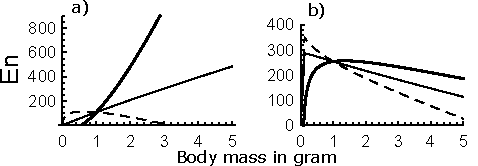
\includegraphics{Fig1}}
\caption{
	Daily net energy gain  $E_n$ as function body mass $z$ for $b_2 = 0.5, 0.8, 1.25$, dashed, thin, thick lines, respectively.
	a) Foraging time $t_f$ is fixed to one hour, b) resource availability $R$ is fixed
}% Add non trivial units later
\label{fig1}
\end{center}
\end{figure}

Let us return to dashed line in \cref{fig1}a.
We found that intermediate optimal body mass only occurs under a restricted condition i.e. $d E_n/dz$ is negative for large value of $z$.
We show the derivation in the supplement but in short we found that resource quality $\varepsilon$ in \cref{eq:eg} needs to be within a certain range (\cref{fig2}a).
If $\varepsilon$ is too low (\cref{fig2}a, e.g. dashed horizontal line below the red shaded region for $z > 3 $), $E_n$ becomes negative (\cref{fig2}, red dashed).
If $\varepsilon$ is too high (\cref{fig2}a, e.g. dashed and solid horizontal lines above the blue shaded region),  $d E_n/dz$ becomes positive leading to a monotonic increase in $E_n$ with respect to $z$ (\cref{fig2}b, dashed and solid blue).
In a more technical term, the range of the $\varepsilon$ allowing intermediate optimal body mass is 
\begin{equation}\label{C1}
	\widetilde{E_n} < \varepsilon < \widetilde{dE_n}.
\end{equation}
where,
\begin{flalign*}
\widetilde{E_n} &= \theta_1 + \theta_2, \\
\widetilde{dE_n} &= \frac{b_2}{b_3} \theta_1  +  \frac{b_1}{b_3} \theta_2.
\end{flalign*}
and $\theta_1 = \frac{a_2}{a_3}  z^{b_2 - b_3}  e^{-E/[k (max(T_w(z_{th}),T_e(t))+ 273.15)]}$ and $\theta_2 =  \frac{a_1}{a_3} z^{b_1- b_3}  e^{-E/[k (T_e(t)+ 273.15)]} (3600 \times24 /t_f -1)$.

The difference between  $\widetilde{E_n}$ and  $\widetilde{d E_n}$ is that in  $\widetilde{dE_n}$, each term of  $\widetilde{E_n}$   is weighted by $\frac{b_2}{b_3}$ and $\frac{b_1}{b_3}$.
Thus, a sufficient condition for optimal mass to be intermediate (\cref{C1}) is that the weights are larger than 1 i.e.  $b_3 < b_1$ ($b_2 \geq b_1$ is always true). 
As temperature increases, the term with the product $\frac{b_1}{b_3}$ becomes larger thus increasing the range of values where \cref{C1} is true (\cref{fig2}a).
The same reasoning can be used in the first paragraph.
If $b_3 > b_2$, $d E_n/dz$ is always positive and $E_n$ becomes an increasing function $z$.
When $b_1 < b_3 < b_2$, \cref{C1} can still be satisfied but require fine tuning of the remaining parameters. %this is such a special case I rather not explore

\begin{figure}
\begin{center}
\scalebox{1.5}{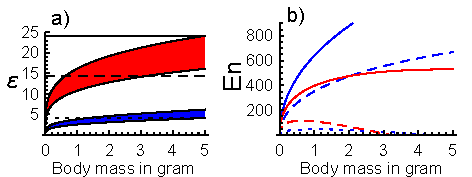
\includegraphics{Fig2}}
\caption{
	a) shaded regions show conditions where $E_n$ is maximized at intermediate value of $z$.
	Resource quality $\varepsilon$ needs to fall inside the shaded regions to satisfy \cref{C1}.
	The upper (lower) limit of the shade region is $\widetilde{dE_n}$ ($\widetilde{E_n}$).  
	b) Different shape of $E_n$ based on a).
	Foraging time $t_f = 1$ hour.
}% Add non trivial units later
\label{fig2}
\end{center}
\end{figure}

\subsection*{Warm-up}
\subsubsection*{Ectotherms}
The ability to warm-up depends on the the surface-to-body ratio.
Because it decreases with increasing body mass, per unit of mass, smaller individual absorbs more energy that larger ones.
However, convection decreases with body mass. 
The effect of these two will generate two patterns.
\cref{fig3}a shows that for free convection, small can warm-up at lower environmental temperature.
The largest need higher temperature not only of the smaller surface-to-body ratio but also because their operative temperature $T_w$ is higher.
\cref{fig3}b shows that when it is windy, warm-up naturally becomes more difficult for any body size.
The optimal body size for warm-up is generally at intermediate value.
If the conductance between the rest-of-the-body and the thorax is low, the effect of body size does not dominate and high environmental temperature is required (\cref{fig3}).

\cref{fig4} shows that it usually takes longer for larger body to warm-up (given they can warm-up).
Evidently, warm-up time is shorter when solar radiation is more intense. 
Here, the blue and the red denotes warm-up starting at sunrise and three hours after sunrise, respectively. 

\subsection*{Influence of temperature}
As in \cref{fig1}, the influence of the exponent of the foraging rate $b_3$ and the amount of resource available defines the optimal body mass (\cref{fig5}).
\cref{fig5}ab show that as long as the exponent $b_3$ is high, large is always optimal.
However, \cref{fig5}c shows that optimal body mass decreases with increasing temperature when $b_3$ is small.
When resource is limited, large cannot be advantageous (\cref{fig5} lower panels).

\cref{fig5} assumes that temperature is constant during the day.
If temperature increases during the day after sunrise, the metabolic costs become higher thus squeeze the thermal niche breadth (defined as the range of temperature with positive net energy gain) to lower value.
In our model, foraging rate defines the upper thermal breadth.

 \subsection*{Combining everything, \cref{fig6,fig7}}
 We summarize here the effects of different components of the model.
 It is important here to note that total foraging time is fixed to 2 hours, thus the longer the warm-up phase, the shorter the time left for foraging.
 One can think of a situation where resources are depleted by the arrival of earlier competitor.  
  Second, the increment in maximum temperature does not depend on temperature at sunrise. 
  For instance when temperature at sunrise is 0 (or 20) degree Celsius, then it peaks at 10 (30) degree Celsius at mid-afternoon.
 \begin{itemize}
 	\item Including warm-up narrows the thermal breadth because
 	\begin{itemize}
	 	\item First, warm-up cannot be completed at low temperature preventing foraging.	
  		\item Second, warm-up takes time and is longer for larger individual (\cref{fig4}. Thus warm-up affects larger individual more and lower thermal breadth is higher for larger individuals
	\end{itemize}  
	\item Adding variation in the temperature (incrementation) decreases thermal breadth because metabolic costs increases. 
	The gain in warm-up ability does not compensate for the increase in energetic cost.
	\item Increasing $b_3$ favors large individuals thus widens thermal breadth of large individuals and narrows the thermal breadth of small individuals.
	\item The first strategy to increase thermal breadth is to wait until there is more solar radiation before warming-up.
	\item The second strategy is to prolong foraging. 
	This last case of course assumes that resources are not highly limiting.
\end{itemize}  
The same pattern is obtained under free or laminar convection. 

\newpage
\subsection*{Remaining figure captions}
\begin{figure}[H]
\begin{center}
%\scalebox{1.25}{\includegraphics{Fig3}}
\caption{
	Minimum environmental temperature required so that warm-up can be completed (maximum time 6 hours).
	Upper (lower) row represents free (laminar convection).
	Left (right) is for default (lower) conductance between thorax and the rest-of-the-body ($K_1$ in \cref{eq:dTr1}.
	Black lines show default value for convection ($K_2$ in \cref{eq:dTr1}), red and blue represent low and convection by one order of magnitude with respect to the default value.
	Solar radiation was increased gradually from 0 to 1320/4 for 6 hours. 
	For the laminar convection,  wind speed is (0.5 m/s).
	Temperature is kept constant
}% Add non trivial units later
\label{fig3}
\end{center}
\end{figure}
 %   
\begin{figure}[H]
\begin{center}
%\scalebox{1.25}{\includegraphics{Fig4}}
\caption{
	Warm-up duration in hour as a function of body size. 
	Warm-up starting at sunrise (3 hours after sunrise) is denoted by blue (red). 
	Thin (thick) line represents default (low) conductance ($K_1$) between the thorax and the rest-of-the-body.
}% Add non trivial units later
\label{fig4}
\end{center}
\end{figure}

\begin{figure}[H]
\begin{center}
%\scalebox{1.25}{\includegraphics{Fig5}}
\caption{
	Change in net energy gain as a function of constant environmental temperature. 
	Thick, thin, dashed, gray lines denote respectively an individual with body mass equals to 0.01, 0.1, 1, 5 gram. 
	Upper row assumes foraging time = 1hour,
	Lower row assume the total amount of resource available is 5 gram.
}% Add non trivial units later
\label{fig5}
\end{center}
\end{figure}
%
\begin{figure}[H]
\begin{center}
%\scalebox{1.25}{\includegraphics{Fig6}}
\caption{
	Change in net energy gain as a function of environmental temperature and the marginal effects of different factors under free convection.
	Line types as in \cref{fig4} except for the thick lines which now represent a body mass of 10 gram.
	See main text under the section \textbf{Combining everything} for more explanation.
}% Add non trivial units later
\label{fig6}
\end{center}
\end{figure}
%
\begin{figure}[H]
\begin{center}
%\scalebox{1.25}{\includegraphics{Fig7}}
\caption{
	Same as in \cref{fig6} but under forced convection.
}% Add non trivial units later
\label{fig7}
\end{center}
\end{figure}


%\subsubsection*{Influence of environmental temperature}
%As in the previous section, the results are represented either assuming a fixed foraging time or a fixed amount of resource.
%In the first case, when $b_3$ is large, largest size is optimal for any environmental temperature (\cref{fig3}a).
%However, when $b_3$ is small, optimal body mass is a decreasing function of temperature (\cref{fig3}b).
%%At high temperature, it is easier to satisfy \cref{C1} as it allows a broader range of  resource quality (\cref{fig1}b).
%%note here than in fig1, we changed $\varepsilon$ and in here $varepsilon$ is fixed but the shaded region is low and narrow
%
%Increasing the cost of warm-up does not change the relationship between optimal body mass and temperature but significantly reduces the thermal niche of each individual (\cref{fig3}c).
%However, thermal niche is not only a function of internal parameters, as the quality of resource ameliorates, the thermal niche of the largest individual broadens (\cref{fig3}d).
%
%In the second case where the amount of resource is fixed, intermediate body mass is optimal (\cref{fig3}e). 
%Largest individuals are limited by resource availability and smaller individual cannot gather enough resource due to limited foraging time (we assumed that foraging cannot exceed 12 hours). % not 100% sure..
%Increasing the cost of warm-up penalizes smallest to medium-size individuals such that largest becomes optimal at low temperature (\cref{fig3}f).
%
%As a general conclusion, for all panels in (\cref{fig3}), irrespective of the conditions, optimal environmental temperature decreases with increasing body mass. 
%Depending on parameters $b_3$ and $R$ or foraging time $t_f$, optimal body mass is the largest (\cref{fig2}a), optimal body mass decreases with temperature \cref{fig2}b, or optimal body mass is at intermediate value \cref{fig2}e.
%The capacity of warm-up limits thermal niche of smaller individuals whereas the amount and quality of resource available limits thermal niche of larger individuals.
%
%\begin{figure}
%\begin{center}
%\scalebox{1.25}{\includegraphics{Fig3}}
%\caption{
%	Panels show daily net energy gain  $E_n$ as function of environmental temperature $T_e(t) = \tau$ for 5 body masses.
%	In a), b), c), and d) Foraging time $t_f$ is fixed to one hour.
%	In e) and f) resource availability is $R$ is fixed to 60 g. 
%	In c) resource quality $\varepsilon$ is higher $14.4$, in the remaining panels (a), b), d), e) and f), $\varepsilon = 8.4$.
%	In c), d), and f), conductance is 14 times higher.
%	Other parameters: $a_2 = 10 \times a_1$, remaining parameters as in \cref{fig1}.
%}% Add non trivial units later
%\label{fig3}
%\end{center}
%\end{figure}
%
%
%\subsection*{Result for the warm-up}
%See appendix for preliminary results
%
%\subsection*{Influence of variable environment temperature}
%...
%The main point here is to look at the influence of fluctuating temperature to make the model results more realistic.



%%Don't read this, I kept in case some recycling is required 
%\subsubsection*{Case 1 = No warm-up}
%For simplicity let us assume that there is no need to warm-up so that $e_w = 0 $ and $t_w =  0$.
%\begin{flalign*}
%	e_r(z) & = \varepsilon a_3 z^{b_3} \times t_f  - \left( \rho a_1 z^{b_2} E_0 Q_{10}^{\frac{\tau}{10}} \times t_f +  a_1 z^{b_1} E_0 Q_{10}^{\frac{\tau}{10}}\times (3600\times24 - t_f) \right) \\
%			& =  z_3^{b_3} \left[  \varepsilon a_3 \times t_f  - \rho a_1  E_0 Q_{10}^{\frac{\tau}{10}} z^{b_2 - b_3} \times t_f -  a_1 z^{b_1- b_3}  E_0 Q_{10}^{\frac{\tau}{10}}\times (3600\times24 - t_f) \right] 
%%			& =  z_3^{b_3} \left[  (\varepsilon a_3  - \rho a_1 Q_{10}^{\frac{\tau}{10}} z^{b_2 - b_3}) \times t_f -  a_1 z^{b_1- b_3} Q_{10}^{\frac{\tau}{10}}\times (3600\times24 - t_f) \right] 
%\end{flalign*}
%Thus, the net energy gain is positive if the term between the square brackets is positive, 
%\begin{equation} \label{eq:C1}
%	\frac{\varepsilon a_3}{ E_0 Q_{10}^{\frac{\tau}{10}}} > \rho a_1  z^{b_2 - b_3} +  a_1 z^{b_1- b_3}  (3600 \times24 /t_f -1)
%\end{equation}
%Net energy gain ($e_r$) increases with body size if $\frac{d e_r}{dz} > 0$, i.e. 
%\begin{equation} \label{eq:C2}
%	\frac{\varepsilon a_3}{ E_0 Q_{10}^{\frac{\tau}{10}}} > \rho a_1  z^{b_2 - b_3} \frac{b_2}{b_3} +  a_1 z^{b_1- b_3}  (3600 \times24 /t_f -1) \frac{b_1}{b_3}.
%\end{equation}
%In contrast, net energy gain ($e_r$) decreases with body size if $\frac{d e_r}{dz} <  0$, i.e. 
%\begin{equation} \label{eq:C3}
%	\frac{\varepsilon a_3}{ E_0 Q_{10}^{\frac{\tau}{10}}} < \rho a_1  z^{b_2 - b_3} \frac{b_2}{b_3} +  a_1 z^{b_1- b_3}  (3600 \times24 /t_f -1) \frac{b_1}{b_3}.
%\end{equation}
%% E: Explain why this situation is of particular interest.  absolute vs proportional/specific energy gain
%Inequations~(\ref{eq:C1}) and~(\ref{eq:C3}) give
%\begin{equation} \label{eq:C4}
%	\rho a_1  z^{b_2 - b_3} +  a_1 z^{b_1- b_3}  (3600 \times24 /t_f -1) < \frac{\varepsilon a_3}{ E_0 Q_{10}^{\tau/10}} < \rho a_1  z^{b_2 - b_3} \frac{b_2}{b_3} +  a_1 z^{b_1- b_3}  (3600 \times24 /t_f -1) \frac{b_1}{b_3},
%\end{equation}
%which is true if $b_2 > b_1 > b_3$ and the middle term is fine tuned.
%Thus, smaller individual may gain more energy than large individuals but under rather restricted conditions.
%If $b_3 > b_2 > b_1$,~(\ref{eq:C1}) implies~(\ref{eq:C2}) and net energy gain increases with body size.
%



%\input{./Appendix_warm-up_derivation.tex }

\bibliography{ref2}
\end{document}
